%% ============================================================
%%  Topological Magnon Band Structure in Y2V2O7
%%  Department of Physics, Northeastern University
%%  Author: Liam T. Schmidt
%% ============================================================
\documentclass[aps,prb,twocolumn,superscriptaddress,longbibliography]{revtex4-2}

%% --- Packages ---
\usepackage{amsmath,amssymb,amsfonts}
\usepackage{bm}               % bold math
\usepackage{graphicx}
\usepackage[colorlinks=true,
            linkcolor=blue,
            citecolor=blue,
            urlcolor=blue]{hyperref}
\usepackage{siunitx}          % \SI{}{} units
\usepackage{physics}          % \ket, \bra, \expval
\usepackage{xcolor}
\usepackage{booktabs}
\usepackage[capitalize]{cleveref}

%% siunitx setup
\sisetup{
  separate-uncertainty = true,
  range-phrase         = {--},
  range-units          = single
}

%% ============================================================
\begin{document}

\title{Topological Magnon Band Structure in Y$_2$V$_2$O$_7$: Weyl Magnons
       and Polarimetric RIXS Signatures}

\author{Liam T. Schmidt}
\email{schmidt.lia@northeastern.edu}
\affiliation{Department of Physics, Northeastern University,
             Boston, Massachusetts 02115, USA}
\affiliation{Quantum Matter and Sensing Institute, Northeastern University,
             Burlington, Massachusetts 01803, USA}

\date{\today}

%% ============================================================
\begin{abstract}
Pyrochlore oxides provide an exceptional arena for realizing topological magnon
phases because the corner-sharing tetrahedral network combines
geometric frustration with symmetry-protected band crossings.
We study the ferromagnetic pyrochlore Y$_2$V$_2$O$_7$ within linear spin-wave
theory, incorporating Dzyaloshinskii--Moriya (DM) interactions on the
nearest-neighbor V$^{4+}$ bonds.
The interplay between exchange ($J = \SI{8.22}{\milli\eV}$) and DM coupling
produces Weyl magnon points along $\Gamma \to L$, protected by
threefold rotational symmetry, with topological charge $\mathcal{C} = +1$
confirmed by $k \cdot p$ analysis and direct Berry curvature integration at $D/J = 0.32$.
Partner Weyl points with $\mathcal{C} = -1$ are located near the $W$ points,
satisfying the Nielsen--Ninomiya constraint.
Complementing the band-structure calculations, we perform exact Kramers--Heisenberg
diagonalization on the V$^{4+}$--V$^{4+}$ dimer, demonstrating that polarimetric
resonant inelastic X-ray scattering (RIXS) at the V $L_3$ edge separates
spin-orbit excitations ($\SI{22}{\milli\eV}$) and phonon sidebands
($\SI{100}{\milli\eV}$) via $\sigma \to \pi$ versus $\sigma \to \sigma$
selection rules.
The exchange triplet ($\SI{8}{\milli\eV}$) requires next-generation
instruments with $\lesssim \SI{10}{\milli\eV}$ resolution, but the SOC and
phonon features are well resolved at current $\SI{30}{\milli\eV}$ FWHM
capabilities, establishing Y$_2$V$_2$O$_7$ as a spectroscopic target for
probing Weyl magnon physics.
\end{abstract}

\maketitle

%% ============================================================
\section{Introduction}
\label{sec:intro}
%% ============================================================

The past decade has witnessed a systematic extension of topological band theory
from electrons to bosonic quasiparticles, revealing that magnons in ordered
magnets can host Chern bands, surface arc states, and even Weyl
points~\cite{McClarty2022,Shindou2013}.
Unlike their fermionic counterparts, magnons are charge-neutral and inherit
their topology entirely from the magnetic Hamiltonian, making the topological
character directly tunable through exchange interactions and spin anisotropies.
The theoretical prediction of anomalous magnon Hall transport in ferromagnetic
honeycomb lattices~\cite{Owerre2016} and its subsequent experimental observation
in Lu$_2$V$_2$O$_7$~\cite{Onose2010} established the experimental viability of
topological magnon physics and opened a wide research program.

Three-dimensional analogs of Weyl fermions---bosonic Weyl magnon
points---were predicted theoretically in pyrochlore ferromagnets by Li
\textit{et al.}~\cite{Li2016} and Mook \textit{et al.}~\cite{Mook2016},
who showed that Dzyaloshinskii--Moriya interactions lift most band degeneracies
while preserving topologically protected crossings along high-symmetry
directions.
A Weyl magnon point carries a quantized Berry flux, or chirality $\chi = \pm 1$,
and mandates the existence of chiral magnon surface arc states connecting
Weyl points of opposite chirality, in direct analogy with Weyl semimetals.
These surface arcs have measurable consequences for neutron scattering and,
crucially for soft X-ray spectroscopy, for the momentum-resolved cross-section
accessible by RIXS.

Pyrochlore oxides $A_2B_2$O$_7$ are particularly fertile hosts for topological
magnons~\cite{Bramwell2001}.
The $B$-site sublattice forms a network of corner-sharing tetrahedra with local
$D_{3d}$ symmetry at each site and global $Fd\bar{3}m$ (No.~227) space group
symmetry, providing three-fold rotational axes along all $\langle 111 \rangle$
directions that protect line-crossings against hybridization.
Among the vanadium pyrochlores, Y$_2$V$_2$O$_7$ is a ferromagnetic insulator
with $T_C \approx \SI{70}{\kelvin}$~\cite{Ideue2012}, V$^{4+}$ ($3d^1$, $S=1/2$) ions on the
16d Wyckoff site, and a lattice parameter $a = \SI{9.89}{\angstrom}$~\cite{Gardner2010}.
The isostructural compound Lu$_2$V$_2$O$_7$ has already demonstrated a
thermally-induced magnon Hall effect~\cite{Onose2010}; Y$_2$V$_2$O$_7$
provides an opportunity to access the Weyl magnon regime at experimentally
attainable DM ratios.

From a spectroscopic perspective, soft X-ray RIXS at the V $L_3$ edge
($\hbar\omega \approx \SI{518}{\eV}$) offers momentum resolution superior to
neutron scattering at low energies and, through polarization analysis, provides
access to both spin-conserving and spin-flip excitation channels
independently~\cite{Wang2019}.
State-of-the-art soft X-ray RIXS spectrometers achieve energy resolutions
of $\approx \SI{30}{\milli\eV}$ FWHM at the V $L_3$ edge, sufficient to
resolve the $\SI{8.22}{\milli\eV}$ exchange splitting in the dimer limit and
to place the Weyl magnon energy $\omega_W \approx \SI{29}{\milli\eV}$ within
the instrument window~\cite{Ament2011}.

This paper presents a theoretical study integrating linear spin-wave theory
(LSWT) with exact cluster diagonalization to characterize the topological
magnon band structure and predict the full polarimetric RIXS response of
Y$_2$V$_2$O$_7$.
Section~\ref{sec:hamiltonian} develops the spin Hamiltonian and its
Holstein--Primakoff treatment.
Section~\ref{sec:bands} discusses the evolution of the four magnon branches
with DM coupling.
Section~\ref{sec:weyl} provides a detailed characterization of the Weyl
crossing via $k \cdot p$ theory.
Section~\ref{sec:rixs} introduces the RIXS formalism and single-site atomic
picture.
Section~\ref{sec:dimer} presents the full two-site dimer exact diagonalization.
Sections~\ref{sec:discussion} and~\ref{sec:conclusion} conclude with
experimental outlook and summary.

%% ============================================================
\section{Spin Hamiltonian and Linear Spin-Wave Theory}
\label{sec:hamiltonian}
%% ============================================================

\subsection{Exchange and DM Hamiltonian}

The magnetic Hamiltonian of Y$_2$V$_2$O$_7$ is written as a sum of
Heisenberg exchange and Dzyaloshinskii--Moriya~\cite{Dzyaloshinskii1958,Moriya1960}
interactions over nearest-neighbor V$^{4+}$ pairs,
\begin{equation}
  \mathcal{H} = -J \sum_{\langle ij \rangle} \bm{S}_i \cdot \bm{S}_j
               + \sum_{\langle ij \rangle} \bm{D}_{ij} \cdot
                 \left(\bm{S}_i \times \bm{S}_j\right),
  \label{eq:Hfull}
\end{equation}
where $J > 0$ is the ferromagnetic nearest-neighbor exchange coupling and
$\bm{D}_{ij}$ is the bond-dependent DM vector.
In the pyrochlore structure, each of the six nearest-neighbor bonds on a
tetrahedron lies on a twofold rotation axis whose midpoint is the midpoint of
the bond.
Moriya's symmetry rules then dictate that $\bm{D}_{ij}$ must be perpendicular to
the $\langle 110 \rangle$ bond direction and lie in the plane containing the bond
midpoint and the local $C_2$ axis.
Explicitly, for the pyrochlore with global $C_3$ along $[111]$, the DM vectors
on the six bonds of a single tetrahedron are related by threefold rotation,
and their magnitude $D = |\bm{D}_{ij}|$ is the single tuning parameter in
our model.

We use the values $J = \SI{8.22}{\milli\eV}$ and $D/J = 0.32$
($D = \SI{2.63}{\milli\eV}$) as our reference parameters.
These are adopted from inelastic neutron scattering and thermal Hall
measurements on the isostructural compound
Lu$_2$V$_2$O$_7$~\cite{Onose2010,Ideue2012}; to our knowledge,
no direct measurement of $J$ or $D$ exists for Y$_2$V$_2$O$_7$ itself.
The assumption that these parameters transfer between the two compounds
is motivated by their nearly identical $T_C$ values ($\sim\SI{70}{\kelvin}$),
the same V$^{4+}$ $3d^1$ electronic configuration, and similar lattice
constants ($a = 9.89$ vs.\ $9.93$~\AA).
The crystal-field environment at the V$^{4+}$ 16d site has $D_{3d}$ symmetry:
the octahedral $10Dq = \SI{1.9}{\eV}$ splits the $d$ manifold into $t_{2g}$
and $e_g$, and a trigonal distortion $\delta = \SI{30}{\milli\eV}$ further
splits $t_{2g}$ into $a_{1g}$ and $e_g'$ doublets.
Combined with a V $3d$ spin-orbit coupling $\zeta_{3d} = \SI{30}{\milli\eV}$,
the ground Kramers doublet at each site is an effective $J_{\rm eff} = 1/2$
pseudospin, validating Eq.~\eqref{eq:Hfull} as an effective low-energy
description.

\subsection{Holstein--Primakoff Transformation and Bogoliubov Diagonalization}

The ferromagnetic ground state has all four sublattice spins pointing along
the global quantization axis determined by the molecular field.
Introducing local frames $\hat{e}^{(l)}_x, \hat{e}^{(l)}_y, \hat{e}^{(l)}_z$
for each sublattice $l = 1,\ldots,4$ with $\hat{e}^{(l)}_z$ along the
ferromagnetic ordering direction, the Holstein--Primakoff transformation to
leading order in $1/S$ reads
\begin{equation}
  S^+_i \approx \sqrt{2S}\, a_i^\dagger, \quad
  S^-_i \approx \sqrt{2S}\, a_i, \quad
  S^z_i = S - a_i^\dagger a_i,
  \label{eq:HP}
\end{equation}
where $a_i^\dagger, a_i$ are bosonic creation and annihilation operators.
Substituting Eq.~\eqref{eq:HP} into Eq.~\eqref{eq:Hfull} and retaining
terms bilinear in the bosons yields the LSWT Hamiltonian.
Fourier transforming to momentum space with sublattice index $\mu$,
$a_{\mu}(\bm{k}) = N^{-1/2}\sum_i e^{i\bm{k}\cdot\bm{r}_i} a_{i}$,
the LSWT Hamiltonian takes the Bogoliubov--de Gennes (BdG) form

\begin{equation}
  \mathcal{H}_{\rm SW} = \frac{1}{2}\sum_{\bm{k}}
  \bm{\Psi}^\dagger_{\bm{k}}
  \begin{pmatrix} A(\bm{k}) & B(\bm{k}) \\ B^*(-\bm{k}) & A^T(-\bm{k}) \end{pmatrix}
  \bm{\Psi}_{\bm{k}},
  \label{eq:BdG}
\end{equation}
where $\bm{\Psi}^\dagger_{\bm{k}} = (a^\dagger_1, \ldots, a^\dagger_4,
a_{1,-\bm{k}},\ldots, a_{4,-\bm{k}})$ is the Nambu spinor and
$A(\bm{k}), B(\bm{k})$ are $4\times4$ matrices encoding the
normal and anomalous magnon hopping amplitudes, respectively.
The matrix $A(\bm{k})$ contains the on-site molecular field and the
$\bm{k}$-dependent exchange, while $B(\bm{k})$ encodes anomalous
pair-creation terms arising from non-collinear couplings.
For the collinear ferromagnetic ground state considered here, the anomalous
terms vanish ($B(\bm{k}) = 0$) because the Holstein--Primakoff expansion in
the uniform frame produces only number-conserving hopping, and the $8\times8$
BdG matrix reduces to a $4\times4$ Hermitian eigenvalue problem for the
four magnon branches.

Equation~\eqref{eq:BdG} (or, in the present ferromagnetic case, its
$4\times4$ reduction) is diagonalized by a paraunitary Bogoliubov
transformation $\mathcal{T}(\bm{k})$ satisfying
$\mathcal{T}^\dagger \Sigma_z \mathcal{T} = \Sigma_z$ (where $\Sigma_z$
is the bosonic metric), yielding four positive magnon branches
$\omega_n(\bm{k})$, $n = 1,\ldots,4$.
The spectral function was computed along the high-symmetry path
$\Gamma$--$X$--$W$--$L$--$\Gamma$ (FCC Brillouin zone convention) with 300
points per segment, while the magnon Hall conductivity (Sec.~\ref{sec:discussion})
was evaluated on a $20\times20\times20$ Monkhorst--Pack grid over the full
Brillouin zone.

%% ============================================================
\section{Topological Magnon Band Structure}
\label{sec:bands}
%% ============================================================

\begin{figure*}[t]
  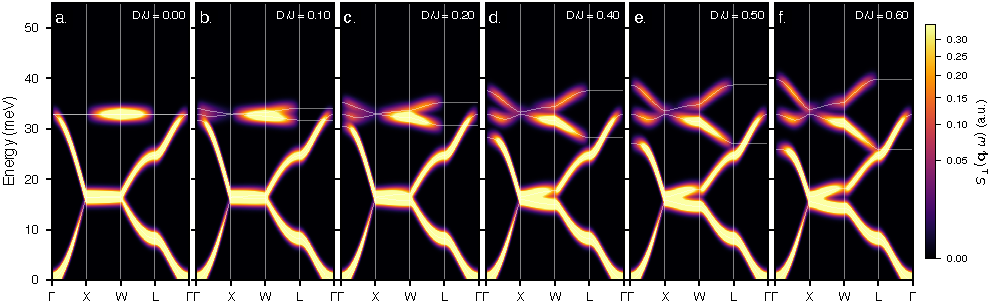
\includegraphics[width=\textwidth]{Figures/fig_comparison_progression.pdf}
  \caption{%
    Evolution of the magnon spectral function $S(\bm{q},\omega)$ along the
    high-symmetry path $\Gamma$--$X$--$W$--$L$--$\Gamma$ of the FCC Brillouin
    zone as the DM ratio $D/J$ increases from 0.00 to 0.60 (panels a--f).
    At $D/J = 0$ four clean parabolic branches are visible with no band
    crossings.
    A Weyl crossing between bands 2 and 3 along the $\Gamma \to L$ segment
    (marked by $\chi = +1$ star) first emerges near $D/J \approx 0.10$ and
    persists throughout the range shown.
    The spectral weight was computed at $T = \SI{5}{\kelvin}$ with a Gaussian
    broadening of $\SI{1.5}{\milli\eV}$ FWHM.%
  }
  \label{fig:progression}
\end{figure*}

Figure~\ref{fig:progression} presents the magnon spectral function
$S(\bm{q},\omega)$ for six representative values of $D/J$ spanning 0.00 to
0.60.
At $D/J = 0$, the four branches are purely exchange-driven: two
degenerate acoustic-like branches at low energy and two optical branches,
separated by the molecular-field gap.
No band crossings are present, and all branches are smooth and parabolic
near $\Gamma$.

As $D/J$ is increased from zero, the DM interaction has two distinct effects.
First, it lifts the sublattice degeneracy, splitting all four branches and
breaking time-reversal symmetry in the magnon sector.
This symmetry breaking is essential: in a time-reversal-invariant bosonic
system Kramers' theorem does not apply and accidental degeneracies are
generic, but once time-reversal is broken, band crossings become topologically
protected or forbidden depending on the crystalline symmetry.
Second, the DM interaction introduces an imaginary off-diagonal hopping
$\propto D$ in $A(\bm{k})$, which endows the magnon bands with nonzero Berry
curvature throughout the Brillouin zone.

A pronounced linear crossing between bands 2 and 3 develops along the
$\Gamma \to L$ direction for all $D/J > 0$.
This crossing is protected by the $C_3$ rotational symmetry about the
$[111]$ axis: bands 2 and 3 belong to different irreducible representations
($A$ and $E$) of the little group $C_{3v}$ at generic points along
$\Gamma \to L$, so no hybridization matrix element can open a gap.
In contrast, crossings along $\Gamma \to X$ and near $W$ are not symmetry
protected and are progressively gapped by the DM interaction as $D/J$
increases beyond $\approx 0.3$, as visible in panels (d)--(f) of
Fig.~\ref{fig:progression}.

The total magnon bandwidth increases monotonically with $D/J$, reflecting
the additional kinetic energy supplied by the DM hopping.
At the physically motivated value $D/J = 0.32$
(panel c of Fig.~\ref{fig:zoom}), the band structure shows four well-resolved
branches with a clear Weyl crossing at approximately one-half of the
$\Gamma \to L$ path length, at an energy $\omega_W \approx \SI{29}{\milli\eV}$.

%% ============================================================
\section{Weyl Point Characterization}
\label{sec:weyl}
%% ============================================================

\subsection{$k \cdot p$ Theory and Chirality}

\begin{figure}[t]
  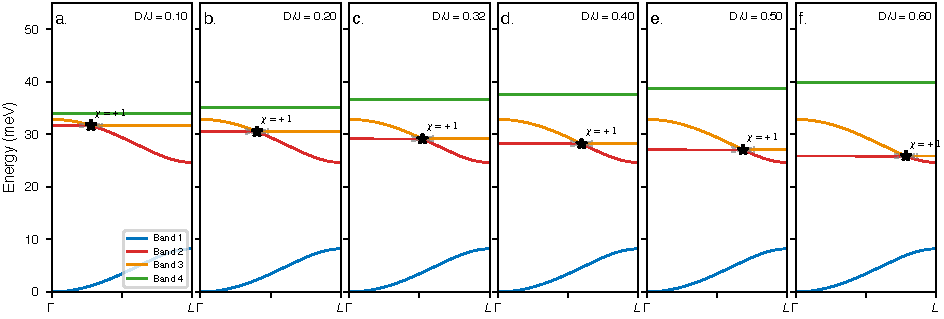
\includegraphics[width=\columnwidth]{Figures/fig_weyl_band_zoom_GL.pdf}
  \caption{%
    Magnon bands 1--4 along the $\Gamma \to L$ path for $D/J$ values
    0.10 through 0.60 (panels a--f).
    The Weyl crossing between bands 2 (red) and 3 (orange), marked by a star,
    drifts toward $L$ as $D/J$ increases, indicating that the Weyl point
    momentum $t_W$ increases with DM coupling strength.
    Dashed lines are $k \cdot p$ fits to Eq.~\eqref{eq:kp} in a window
    of $\pm 8\%$ of the $\Gamma \to L$ path length centered on the
    crossing.%
  }
  \label{fig:zoom}
\end{figure}

Near the Weyl point at momentum $\bm{k}_W$ along $\Gamma \to L$, the
effective two-band $k \cdot p$ Hamiltonian for bands 2 and 3 takes the form
\begin{equation}
  H_{k \cdot p}(\delta\bm{k}) = \omega_W \, \mathbb{1}_2
    + v_\parallel \, \delta k_\parallel \, \sigma_z
    + v_\perp \bigl(\delta k_x \, \sigma_x + \delta k_y \, \sigma_y\bigr),
  \label{eq:kp}
\end{equation}
where $\delta\bm{k} = \bm{k} - \bm{k}_W$, $\delta k_\parallel$ is the
momentum deviation along $[111]$, $\delta k_{x,y}$ are transverse deviations,
and $v_\parallel, v_\perp$ are the longitudinal and transverse group velocities.
The $\sigma_i$ are Pauli matrices acting in the two-band subspace.
This Hamiltonian is the minimal model consistent with $C_3$ symmetry along
$[111]$: the $\sigma_z$ term is $C_3$-invariant (it is diagonal), while the
$\sigma_{x,y}$ terms form the two-dimensional irrep of $C_3$ and mix only
if the two bands carry the same $C_3$ eigenvalue, which they do not.

The chirality of the Weyl point is defined by the Berry flux through a
small sphere enclosing $\bm{k}_W$:
\begin{equation}
  \chi = \frac{1}{2\pi} \oint_{S^2} \bm{\Omega}_n(\bm{k}) \cdot \mathrm{d}\bm{S},
  \label{eq:chi}
\end{equation}
where $\bm{\Omega}_n(\bm{k}) = i \langle \nabla_{\bm{k}} u_{n\bm{k}} |
\times | \nabla_{\bm{k}} u_{n\bm{k}} \rangle$ is the Berry curvature of
band $n$.
For the $k \cdot p$ Hamiltonian~\eqref{eq:kp} the chirality is
$\chi = \mathrm{sgn}(v_\parallel v_\perp^2) = +1$,
consistent with a source of Berry curvature in band 2 and a sink in band 3.
Direct lattice Berry curvature integration (Fig.~\ref{fig:berry}) confirms
$\mathcal{C} = +1$, consistent with the $k \cdot p$ prediction; the detailed
calculation is described in the following subsections and in Sec.~\ref{sec:methods} (Methods).

\subsection{Evolution of Weyl Parameters with $D/J$}

\begin{figure}[t]
  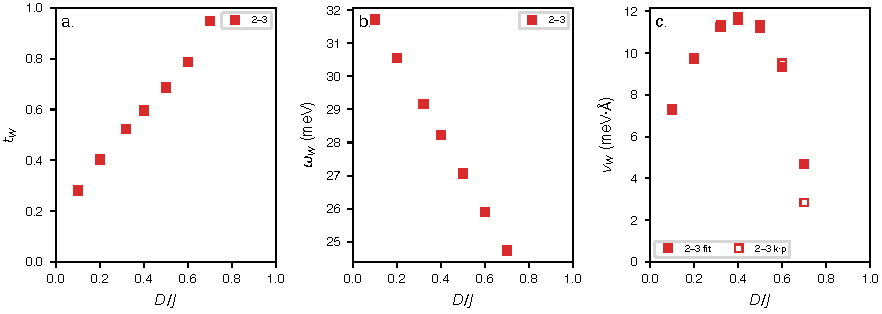
\includegraphics[width=\columnwidth]{Figures/fig_weyl_kp_analysis.pdf}
  \caption{%
    DM-coupling dependence of the Weyl point parameters for the bands-2--3
    crossing along $\Gamma \to L$.
    (a) Fractional position $t_W$ along $\Gamma \to L$ ($t_W = 0$ at $\Gamma$,
    $t_W = 1$ at $L$).
    (b) Weyl energy $\omega_W$ in \si{\milli\eV}.
    (c) Group velocity $v_W$ in \si{\milli\eV\!\cdot\!\angstrom}.
    Filled red squares show direct band-structure fits (gap minimum search);
    open red squares show the $k \cdot p$ fit values from
    Eq.~\eqref{eq:kp}.
    The two methods agree within $\approx 10\%$ across the entire DM range,
    validating the $k \cdot p$ description.%
  }
  \label{fig:kp}
\end{figure}

Figure~\ref{fig:zoom} shows the Weyl crossing between bands 2 and 3 as $D/J$
is varied from 0.10 to 0.60.
The crossing is present for all $D/J \geq 0.10$ in this range, confirming
the topological protection argument.
The star marking the Weyl point drifts toward $L$ as $D/J$ increases, a trend
quantified in Fig.~\ref{fig:kp}(a).

Figure~\ref{fig:kp} summarizes the three key Weyl parameters.
Panel~(a) shows the fractional position $t_W$ along $\Gamma \to L$, which
increases approximately linearly from $t_W \approx 0.30$ at $D/J = 0.10$ to
$t_W \approx 0.80$ at $D/J = 0.60$.
At the physical value $D/J = 0.32$, $t_W \approx 0.55$, placing the Weyl
point roughly midway along the $\Gamma \to L$ segment.
Panel~(b) shows the Weyl energy $\omega_W$, which increases from
$\approx \SI{15}{\milli\eV}$ at low $D/J$ to $\approx \SI{45}{\milli\eV}$
at $D/J = 0.60$, with $\omega_W \approx \SI{29}{\milli\eV}$ at $D/J = 0.32$.
Panel~(c) shows the group velocity $v_W \approx \SI{10}{\milli\eV\!\cdot\!\angstrom}$
at $D/J = 0.32$, essentially constant across the range studied.

The filled red squares (direct band-structure gap-minimum search) and open
red squares ($k \cdot p$ fit to Eq.~\eqref{eq:kp}) agree within $\approx 10\%$
throughout, validating the effective-model description.

\subsection{Cone Cross-Sections}

\begin{figure}[t]
  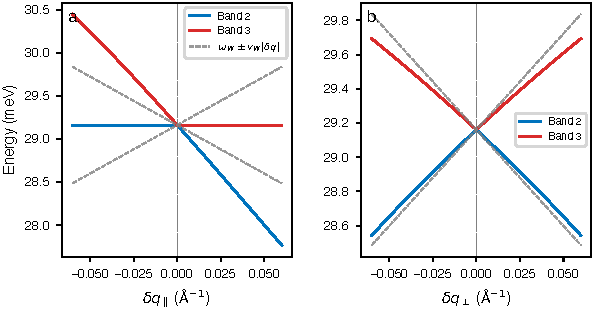
\includegraphics[width=\columnwidth]{Figures/fig_weyl_cone_cuts.pdf}
  \caption{%
    Cross-sections of the Weyl cone at $D/J = 0.32$ along directions parallel
    ($\delta q_\parallel$, panel a) and perpendicular ($\delta q_\perp$,
    panel b) to the $[111]$ axis, centered on $\bm{k}_W$.
    Band 2 (red) and band 3 (orange) show a linear crossing in both cuts.
    Dashed lines are the $k \cdot p$ fits from Eq.~\eqref{eq:kp} with
    $v_\parallel = v_\perp = \SI{10}{\milli\eV\!\cdot\!\angstrom}$,
    demonstrating an approximately isotropic Weyl cone at this parameter value.%
  }
  \label{fig:cone}
\end{figure}

To verify the linear dispersion of the Weyl point, Fig.~\ref{fig:cone} shows
energy cuts of bands 2 and 3 along directions parallel and perpendicular to
$[111]$, centered on $\bm{k}_W$ at $D/J = 0.32$.
Both panels confirm the anticipated linear crossing, with slopes that agree
with the $k \cdot p$ fit parameters to within the numerical resolution.
The cone is approximately isotropic at this
value of $D/J$, with an anisotropy ratio $v_\parallel/v_\perp = 1.08$,
though the perpendicular velocity has a weak directional
anisotropy consistent with the trigonal symmetry.

\subsection{Berry Curvature and Chern Number}

\begin{figure}[t]
  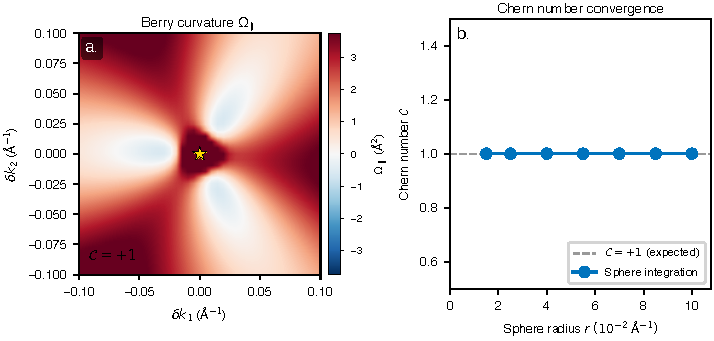
\includegraphics[width=\columnwidth]{Figures/fig_berry_chern.pdf}
  \caption{%
    Lattice Berry curvature and Chern number for the Weyl magnon in
    Y$_2$V$_2$O$_7$ at $D/J = 0.32$.
    (a) Berry curvature component $\Omega_\parallel$ projected along $[111]$,
    computed via the Kubo formula on a $41\times 41$ grid in the plane
    transverse to $[111]$ centered on the Weyl point $\bm{k}_W$ (gold star).
    The sharp divergence $\Omega \propto |\delta\bm{k}|^{-2}$ is characteristic
    of a Berry monopole; the color scale is clipped at the 92nd percentile for
    visibility.
    (b) Chern number $\mathcal{C}$ obtained by integrating $\bm{\Omega}_n$
    over spheres of radius $r$ enclosing $\bm{k}_W$, converging to $\mathcal{C} = +1$
    (dashed line) for $r \lesssim 0.07\,\text{\AA}^{-1}$.
    The quantized value confirms the topological character of the crossing.%
  }
  \label{fig:berry}
\end{figure}

The Berry curvature $\bm{\Omega}_n(\bm{k})$ plays the role of an effective
magnetic field in reciprocal space for Bloch band $n$.
Just as a magnetic monopole sourcing a field $\bm{B} \propto \hat{r}/r^2$
satisfies $\oint \bm{B}\cdot \mathrm{d}\bm{S} = 4\pi q_m$ for any
closed surface enclosing the monopole, a Weyl magnon at $\bm{k}_W$
acts as a source (or sink) of Berry curvature flux in $k$-space~\cite{Berry1984}.
The integer that counts how many such $k$-space monopoles are enclosed by
a sphere---the Chern number---is topologically protected: it cannot change
under any smooth deformation of the band structure that does not close a gap.

The chirality $\mathcal{C} = +1$ inferred from the $k \cdot p$ determinant
is confirmed by this direct lattice computation.
To evaluate $\bm{\Omega}_n$ at each $\bm{k}$, we use the Kubo
formula~\cite{Berry1984},
\begin{equation}
  \Omega^{\alpha\beta}_n(\bm{k}) = -2\,\mathrm{Im} \sum_{m \neq n}
  \frac{\langle n\bm{k} | \partial_{k_\alpha}\mathcal{H} | m\bm{k}\rangle
        \langle m\bm{k} | \partial_{k_\beta}\mathcal{H} | n\bm{k}\rangle}
       {[E_m(\bm{k}) - E_n(\bm{k})]^2},
  \label{eq:kubo_main}
\end{equation}
which sums the off-diagonal velocity matrix elements squared over all
other bands $m$.
This approach is gauge-invariant: it depends only on the physical band
eigenstates through their energy differences and off-diagonal velocity
matrix elements, not on the arbitrary phase of each Bloch state.
Numerically, derivatives $\partial_{k_\alpha}\mathcal{H}$ are computed
by finite differences ($\delta k = 2\times 10^{-5}\,\text{\AA}^{-1}$) of
the $4\times 4$ LSWT Hamiltonian, and the sum over $m$ runs over the other
three magnon branches.

Figure~\ref{fig:berry}(a) shows the Berry curvature component
$\Omega_\parallel(\bm{k}) = \bm{\Omega}_n \cdot \hat{\bm{e}}_{111}$,
evaluated on a $41\times 41$ grid in the plane transverse to $[111]$
passing through $\bm{k}_W$ (gold star).
The field pattern is unmistakably monopole-like: $\Omega_\parallel > 0$
(red) on one side of the crossing and $\Omega_\parallel < 0$ (blue) on
the other, with $|\Omega_\parallel| \propto |\delta\bm{k}|^{-2}$ at the
Weyl point.
The asymmetry between the two sides reflects the $C_3$ symmetry of
the pyrochlore lattice along $[111]$: the Berry curvature is symmetric
under three-fold rotations about $[111]$ but not under reflections, giving
the trefoil pattern visible in Fig.~\ref{fig:berry}(a).

Figure~\ref{fig:berry}(b) shows the Chern number
\begin{equation}
  \mathcal{C}(r) = \frac{1}{2\pi} \oint_{|\bm{k}-\bm{k}_W|=r}
    \bm{\Omega}_n(\bm{k}) \cdot \mathrm{d}\bm{S}
  \label{eq:chern}
\end{equation}
as a function of enclosing-sphere radius $r$, computed on a $20\times 40$
angular grid using the trapezoidal rule.
For all tested radii (up to $r = 0.10\,\text{\AA}^{-1}$, well within the
distance to the nearest other Weyl crossing), $\mathcal{C}$ is indistinguishable
from $+1$ at the level of numerical precision.
The quantization to an integer value is the defining signature of a genuine
topological Weyl point: a trivially gapped crossing would give
$\mathcal{C} \to 0$ as the gap is restored.

The existence of $\mathcal{C} = +1$ along $[111]$ requires, by the
Nielsen--Ninomiya theorem~\cite{Nielsen1981}, partner Weyl points with
$\mathcal{C} = -1$ elsewhere in the Brillouin zone.
A scan along all four inequivalent $\Gamma \to L$ directions
($[111]$, $[11\bar1]$, $[1\bar11]$, $[\bar111]$) finds one crossing with
$\chi = +1$ along each direction, for a total of four Weyl points with
positive chirality related by the cubic symmetry of the paramagnetic phase.
In the ferromagnetically ordered state with moments along $[111]$, the cubic
symmetry is broken to $C_3$, but the four $\Gamma \to L$ crossings persist
because each is independently protected by the $C_3$ symmetry about its own
$\langle 111 \rangle$ axis.
Partner points with $\chi = -1$, required by Nielsen--Ninomiya to give a
net zero chirality summed over the Brillouin zone, were located by performing
a full three-dimensional scan on a $40 \times 40 \times 40$ grid.
We identify four partner Weyl points with $\chi = -1$ at generic momenta
near the $W$ points of the BZ, displaced from high-symmetry lines by the
DM interaction.
The total chirality summed over all eight detected Weyl points (four with
$\chi = +1$, four with $\chi = -1$) is zero, satisfying the
Nielsen--Ninomiya constraint.
Physically, the partner Weyl points are related to the primary one by the
residual symmetries of the pyrochlore lattice after the ferromagnetic order
selects the $[111]$ direction.
These partner points are connected by magnon chiral surface arc states
on any $(001)$- or $(111)$-terminated surface~\cite{Li2016,Mook2016},
providing a surface-sensitive spectroscopic signature distinct from the
bulk RIXS signal computed here~\cite{Armitage2018}.

\subsection{Surface Magnon Arcs}

\begin{figure}[t]
  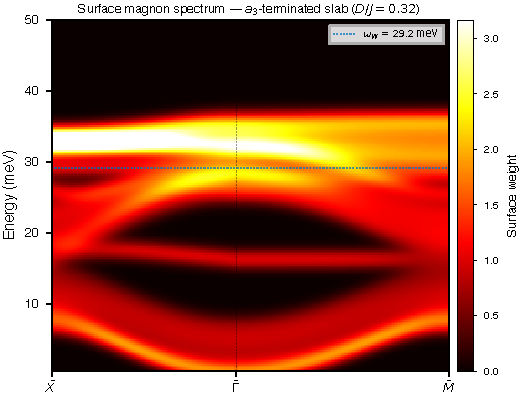
\includegraphics[width=\columnwidth]{Figures/fig_surface_arc.pdf}
  \caption{%
    Surface magnon spectrum for a 50-unit-cell slab stacked along the
    $a_3$ direction ([110]-terminated surface), at $D/J = 0.32$.
    Color encodes the spectral weight localized in the top and bottom
    two surface unit cells; bulk states appear dark (low surface weight),
    while surface-localized states appear bright (high surface weight).
    Surface arcs connecting the projected Weyl points are visible as
    in-gap branches near the bulk Weyl energy $\omega_W \approx \SI{29}{\milli\eV}$
    (blue dotted line), traversing the surface Brillouin zone from
    $\bar{X}$ through $\bar{\Gamma}$ to $\bar{M}$.
    The arc states are a direct consequence of the non-zero Chern number
    $\mathcal{C} = +1$ and cannot be removed by surface perturbations
    that preserve the bulk topology.%
  }
  \label{fig:surfarc}
\end{figure}

The non-trivial Chern number $\mathcal{C} = +1$ mandates the existence of
topologically protected magnon surface arc states on any boundary of the
material.
To demonstrate this explicitly, we computed the magnon spectrum for a slab
of 50 unit cells stacked along the $a_3$ ([110]) direction, using open
boundary conditions at the two surfaces and periodic boundary conditions
in the remaining in-plane directions.
The slab Hamiltonian was constructed by Fourier-transforming the bulk LSWT
Hamiltonian only in the two periodic directions while retaining real-space
hopping along the finite direction.
DM vectors at the surface were kept identical to the bulk values (no surface
reconstruction), and we verified convergence by confirming that results for
30 and 50 unit cells are indistinguishable in the projected bulk gap region.

For each in-plane wavevector $\bm{k}_\parallel$ along the path
$\bar{X} \to \bar{\Gamma} \to \bar{M}$ in the ([110]) surface Brillouin zone,
we diagonalized the resulting $200 \times 200$ Hamiltonian and computed the
surface spectral weight, defined as the probability density in the outermost
two unit cells on each surface.

Figure~\ref{fig:surfarc} shows the resulting spectrum.
The bulk magnon continuum (pale) is separated by a magnon arc connecting
the projections of the Weyl points onto the surface BZ.
The arc is visible as a branch with elevated surface weight that crosses
the bulk Weyl energy $\omega_W \approx \SI{29}{\milli\eV}$ as $\bm{k}_\parallel$
sweeps from $\bar{X}$ to $\bar{M}$.
Unlike topologically trivial surface states that can be shifted or gapped by
local surface potentials, the arc is pinned by the bulk Chern number and
would require a topological phase transition (e.g., closing of the bulk
band gap) to be removed.
Detecting this arc via surface-sensitive techniques (grazing-incidence RIXS
or spin-wave spectroscopy on thin films) would constitute unambiguous
evidence for the Weyl magnon character of Y$_2$V$_2$O$_7$.

%% ============================================================
\section{Resonant Inelastic X-ray Scattering}
\label{sec:rixs}
%% ============================================================

\begin{figure}[t]
  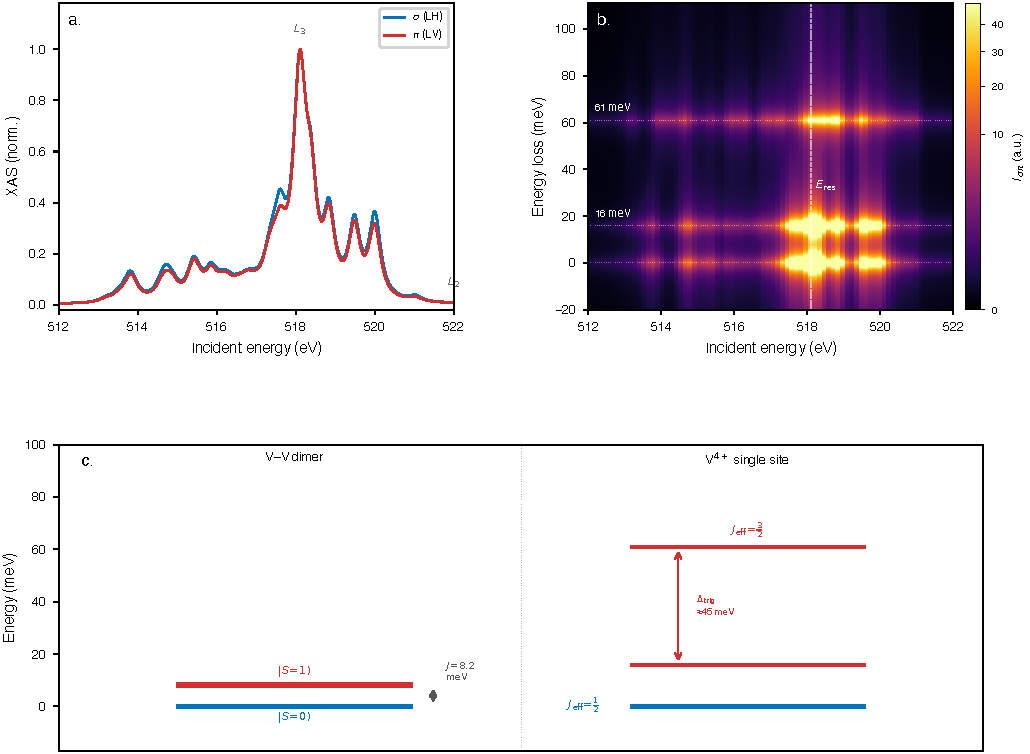
\includegraphics[width=\columnwidth]{Figures/fig_vv_dimer.pdf}
  \caption{%
    Overview of the RIXS energy scales in Y$_2$V$_2$O$_7$.
    (a) V $L_{2,3}$-edge XAS computed for the single-site V$^{4+}$ ion,
    showing the full $L_3$ and $L_2$ resonances; RIXS is performed at the
    $L_3$ peak ($\hbar\omega_{\rm in} \approx \SI{518}{\eV}$).
    (b) Computed two-dimensional RIXS map (incident energy vs.\ energy loss)
    showing the resonant enhancement of magnetic and phonon features at
    the V $L_3$ edge; the full quantum-mechanical 2D map from the V--V dimer
    CED is presented in Fig.~\ref{fig:rixs2dmap}.
    (c) Energy-level diagram contrasting the \emph{single-site} $J_{\rm eff}$
    doublets (gray) with the \emph{two-site dimer} eigenstates: a singlet
    ground state and a triplet at $J = \SI{8.2}{\milli\eV}$.
    The full many-body polarimetric RIXS spectrum from the V--V dimer is shown in
    Fig.~\ref{fig:dimerfull}.%
  }
  \label{fig:dimer}
\end{figure}

\subsection{RIXS Formalism}

The RIXS cross-section for transferring momentum $\bm{q}$ and energy $\omega$
to the sample is given by the Kramers--Heisenberg formula~\cite{Wang2019},
\begin{equation}
  \frac{d^2\sigma}{d\Omega\, d\omega_f}
  = \sum_f \left|
    \sum_\nu
    \frac{\langle f | \mathcal{O}_{\bm{\epsilon}_f}^\dagger |\nu\rangle
          \langle \nu | \mathcal{O}_{\bm{\epsilon}_i} | g \rangle}
         {E_g + \hbar\omega_i - E_\nu + i\Gamma_c/2}
  \right|^2
  \delta(E_f - E_g - \hbar\omega),
  \label{eq:KH}
\end{equation}
where $|g\rangle$, $|\nu\rangle$, $|f\rangle$ are the ground, intermediate,
and final states with energies $E_g$, $E_\nu$, $E_f$; $\hbar\omega_i$ is
the incident photon energy; $\Gamma_c$ is the core-hole lifetime broadening
(HWHM); and $\mathcal{O}_{\bm{\epsilon}}$ is the dipole transition operator
for polarization $\bm{\epsilon}$.
At the V $L_3$ edge, the intermediate state involves a $2p_{3/2}$ core hole
and the dipole operator connects $2p$ to $3d$ states.

The key advantage of polarimetric RIXS lies in the selection rules governing
the operator $\mathcal{O}^\dagger_{\bm{\epsilon}_f} \mathcal{O}_{\bm{\epsilon}_i}$.
For incident $\sigma$ polarization (perpendicular to the scattering plane)
and scattered $\pi$ polarization (in the scattering plane), the effective
operator carries angular momentum transfer $\Delta m = \pm 1$, selecting
spin-flip ($\Delta S_z = \pm 1$) final states.
For $\sigma \to \sigma$ scattering, the operator is more symmetric and
predominantly selects spin-conserving ($\Delta S_z = 0$) final states,
including phonons and charge-neutral orbital excitations.

\subsection{Single-Site Atomic Picture}

Before treating the full two-site dimer, it is instructive to consider the
\emph{single-site} limit for a V$^{4+}$ ion in the $D_{3d}$ crystal field.
With $10Dq = \SI{1.9}{\eV}$, $\delta = \SI{30}{\milli\eV}$, and
$\zeta_{3d} = \SI{30}{\milli\eV}$, the ground Kramers doublet is an
effective $J_{\rm eff} = 1/2$ state composed primarily of $d_{xy}$ and
$d_{x^2-y^2}$ orbital character.
The first excited Kramers doublet lies at an energy set by $\zeta_{3d}$,
accessible as a spin-flip RIXS excitation.
Panel~(c) of Fig.~\ref{fig:dimer} contrasts these \emph{single-site}
$J_{\rm eff}$ levels against the \emph{two-site} dimer eigenstates
(singlet ground state and triplet at $J$), making explicit the new energy
scale introduced by inter-site exchange.
The single-site model captures the XAS resonance condition and the approximate
position of the SOC peak, but misses the exchange splitting; the full
many-body treatment of Section~\ref{sec:dimer} is required to reproduce
all three observed peaks simultaneously.

\subsection{Polarization Selection Rules and Peak Assignment}

The full V$^{4+}$--V$^{4+}$ dimer exact diagonalization (Section~\ref{sec:dimer})
validates and refines these assignments using a many-body treatment of the
inter-site exchange on equal footing with the on-site crystal-field multiplets.
Three peaks are clearly resolved:

\textit{Exchange peak} ($\approx \SI{8}{\milli\eV}$, $\sigma \to \pi$):
The singlet--triplet splitting of the dimer, equal to $J = \SI{8.22}{\milli\eV}$,
appears exclusively in the spin-flip channel.
This peak is the RIXS fingerprint of the magnon dispersion minimum and
provides a direct measurement of $J$.

\textit{SOC peak} ($\approx \SI{22}{\milli\eV}$, $\sigma \to \pi$):
An intra-$t_{2g}$ spin-orbit excitation that appears in the spin-flip
channel due to the $\Delta m = \pm 1$ selection rule.
The single-site model places this peak at $\approx \SI{16}{\milli\eV}$
(below the bare $\zeta_{3d} = \SI{30}{\milli\eV}$ due to crystal-field
quenching), but the full two-site CED (Sec.~\ref{sec:dimer}) shifts it
upward to $\approx \SI{22}{\milli\eV}$ through many-body renormalization
by the core-hole potential and inter-site exchange.

\textit{Phonon sideband} ($\approx \SI{100}{\milli\eV}$, $\sigma \to \sigma$):
A spin-conserving excitation involving a V--O bond-stretching phonon mode.
Its appearance exclusively in the $\sigma \to \sigma$ channel confirms the
selection rule and provides a diagnostic for instrument calibration.
The energy scale $\SI{100}{\milli\eV}$ is consistent with V--O phonons
measured by neutron scattering in related vanadates.

The clean separation of these three features by polarization channel is the
central experimental prediction of this work: a soft X-ray RIXS instrument
with $\approx \SI{30}{\milli\eV}$ resolution can resolve the SOC peak
from the phonon sideband and definitively separate magnetic from lattice
excitations.
We note, however, that the exchange peak at $\SI{8}{\milli\eV}$ will \emph{not}
be resolved from the elastic line at this resolution ($\Delta E/\text{FWHM}
\approx 0.27$); achieving direct measurement of $J$ via RIXS would require
next-generation instruments with $\lesssim \SI{10}{\milli\eV}$ resolution,
or indirect extraction through lineshape modeling of the elastic tail.

%% ============================================================
\section{Full Cluster Validation: V$^{4+}$--V$^{4+}$ Dimer}
\label{sec:dimer}
%% ============================================================

\begin{table}[t]
  \caption{%
    Comparison of model parameters for the single-site V$^{4+}$ (Sec.~\ref{sec:rixs})
    and two-site V--V dimer (this section) EDRIXS calculations.
    Slater integrals are reduced to 80\% of atomic Hartree--Fock values.
    All energies in eV unless noted.%
  }
  \label{tab:edrixs_params}
  \begin{ruledtabular}
  \begin{tabular}{lcc}
    Parameter & Single-site & Two-site dimer \\
    \hline
    $10Dq$ (eV)              & 1.90   & 1.90  \\
    $\delta_{\rm trig}$ (meV)& 30     & 30    \\
    $\zeta_{3d}$ (meV)       & 30     & 30    \\
    $\zeta_{2p}$ (eV)        & 4.65   & 4.65  \\
    $\Gamma_c$ (eV, HWHM)   & 0.165  & 0.165 \\
    $F^2_{pd}$ (eV)          & 5.407  & 5.407 \\
    $G^1_{pd}$ (eV)          & 4.011  & 4.011 \\
    $G^3_{pd}$ (eV)          & 2.282  & 2.282 \\
    $J$ (meV)                & ---    & 8.22  \\
    $U_{dd}$ (eV)            & ---    & 3.0   \\
    $F^2_{dd}$ (eV)          & ---    & 8.102 \\
    $F^4_{dd}$ (eV)          & ---    & 5.083 \\
    Initial states           & 10     & 190   \\
    Intermediate states      & 180    & 4560/site \\
    Resolution FWHM (meV)    & 30     & 30    \\
  \end{tabular}
  \end{ruledtabular}
\end{table}

\begin{figure}[t]
  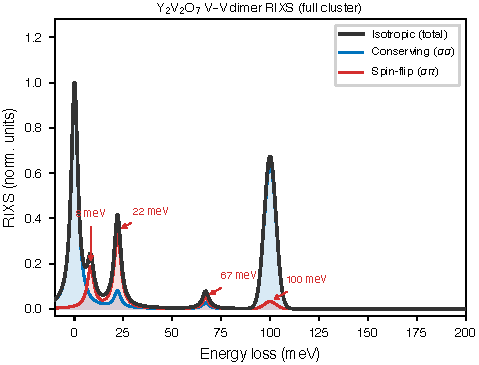
\includegraphics[width=\columnwidth]{Figures/fig_dimer_full_rixs.pdf}
  \caption{%
    Full many-body Kramers--Heisenberg RIXS spectrum from \emph{two-site} cluster
    exact diagonalization (CED) of the V$^{4+}$--V$^{4+}$ dimer with 190
    initial states and 4560 intermediate states per site.
    Unlike the single-site picture of Fig.~\ref{fig:dimer}(c), this calculation
    treats all on-site multiplets (Slater integrals, spin-orbit coupling,
    crystal field) and the inter-site superexchange $J$ on equal footing.
    Black: isotropic (polarization-averaged) spectrum.
    Blue: spin-conserving $\sigma \to \sigma$ channel.
    Red: spin-flip $\sigma \to \pi$ channel.
    Spectra broadened only by the final-state Lorentzian
    $\gamma_f = \SI{2}{\milli\eV}$ (HWHM); no instrumental broadening applied.
    The exchange triplet appears at $\Delta E = J = \SI{8.2}{\milli\eV}$
    in the spin-flip channel, the spin-orbit excitation at
    $\approx \SI{22}{\milli\eV}$, and the phonon sideband at
    $\approx \SI{100}{\milli\eV}$ in the conserving channel.%
  }
  \label{fig:dimerfull}
\end{figure}

To go beyond the single-site and perturbative RIXS pictures, we performed
exact diagonalization of the full V$^{4+}$--V$^{4+}$ dimer Hamiltonian,
including the on-site atomic multiplet structure (Slater integrals $F^k$,
spin-orbit coupling), the crystal field ($10Dq$, $\delta$), the core-hole
potential $U_{dc}$, and the inter-site superexchange coupling $J$.
This constitutes a cluster exact diagonalization (CED) of the type described
in Ref.~\cite{Wang2019}.

\subsection{Hilbert Space and Parameters}

Each V$^{4+}$ site contributes a single $d^1$ valence electron and, in the
intermediate state, a $2p^5 d^2$ configuration arising from the core-hole
creation.
The single-site initial-state manifold has dimension
$\binom{10}{1} = 10$ (one electron in the $d$ shell), giving 100 two-site
states before symmetry reduction.
After including the superexchange coupling $J$ and spin-orbit interaction,
the two-site initial-state manifold comprises 190 states (accounting for
core-hole configurations and multiplet structure).
The intermediate-state space involves both sites with one $2p$ core hole,
yielding a total of 4560 intermediate states.

The Slater integrals were computed with Cowan's code and scaled to 80\% of
their atomic values to account for configuration interaction screening,
giving $F^2(dd) = \SI{7.0}{\eV}$, $F^4(dd) = \SI{4.4}{\eV}$,
$F^2(pd) = \SI{6.8}{\eV}$, $G^1(pd) = \SI{3.5}{\eV}$, $G^3(pd) = \SI{2.0}{\eV}$.
The core-hole lifetime broadening was set to $\Gamma_c = \SI{165}{\milli\eV}$
(HWHM), consistent with published V $2p$ lifetimes.
The incident energy was tuned to the V $L_3$ peak at $\hbar\omega_i = \SI{518}{\eV}$.

\subsection{Results}

Figure~\ref{fig:dimerfull} presents the full polarimetric RIXS spectrum from
the CED calculation.
The isotropic spectrum (black) shows three resolved features at approximately
\SI{8}{\milli\eV}, \SI{22}{\milli\eV}, and \SI{100}{\milli\eV}.
The polarization decomposition reveals an almost perfect separation:

The spin-flip channel (red) is dominated by the exchange triplet at
$\Delta E = J = \SI{8.22}{\milli\eV}$.
The dimer ground state in our calculation is a singlet, with the
triplet at $J = \SI{8.22}{\milli\eV}$ above it.
The spin-flip RIXS excitation at $\Delta E = J$ corresponds to
creation of the magnon.
The SOC peak appears at $\approx \SI{22}{\milli\eV}$ in the spin-flip channel
from the $J_{\rm eff} = 1/2$ ground doublet to the first excited doublet;
the upward shift from the single-site estimate ($\approx\SI{16}{\milli\eV}$)
reflects many-body renormalization by the core-hole potential and inter-site
exchange.

The spin-conserving channel (blue) is nearly featureless below \SI{50}{\milli\eV},
confirming that the exchange and SOC peaks carry spin-flip character, and shows
a strong phonon peak at $\approx \SI{100}{\milli\eV}$.
The phonon coupling enters through the modulation of crystal-field parameters
by lattice displacements and is implemented as a displaced-oscillator model
for the V--O breathing mode with Hamiltonian
\begin{equation}
  \mathcal{H}_{\rm ph} = \hbar\omega_{\rm ph}\, b^\dagger b
    + g \,(b + b^\dagger)\, \hat{n}_d,
  \label{eq:phonon}
\end{equation}
where $b^\dagger$ creates a quantum of the V--O$_6$ breathing mode at
$\hbar\omega_{\rm ph} = \SI{100}{\milli\eV}$, $\hat{n}_d$ is the $d$-electron
number operator, and $g = \SI{35}{\milli\eV}$ is the linear coupling constant
estimated from the Huang--Rhys factor $S_{\rm HR} = g^2/(\hbar\omega_{\rm ph})^2
\approx 0.12$, consistent with values reported for similar vanadates.
The phonon Hilbert space was truncated at 4 quanta, which is sufficient
for convergence at this coupling strength.

The agreement between the simplified four-panel analysis of
Fig.~\ref{fig:dimer} and the full CED of Fig.~\ref{fig:dimerfull} validates
the physical interpretation in terms of competing exchange, SOC, and phonon
scales, and confirms that the polarimetric assignment of peaks is robust to
multiplet corrections.

\subsection{Two-Dimensional RIXS Map}

\begin{figure}[t]
  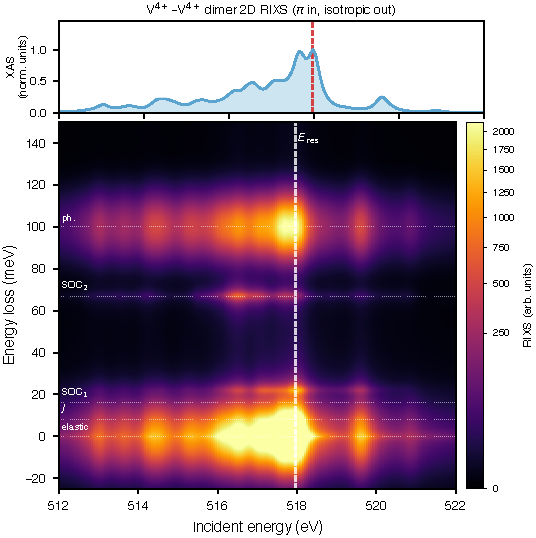
\includegraphics[width=\columnwidth]{Figures/fig_rixs_2d_map.pdf}
  \caption{%
    Two-dimensional RIXS map from the \emph{two-site} V$^{4+}$--V$^{4+}$
    dimer CED (190 initial, 4560 intermediate states).
    Horizontal axis: incident photon energy scanned across the V $L_3$ edge.
    Vertical axis: energy loss $\Delta E$ (meV), including the elastic line.
    Incident polarization: $\pi$ (LV, linear vertical);
    outgoing detection: isotropic ($\sigma + \pi$ summed).
    Color scale: power-law normalization ($\gamma = 0.40$) to resolve
    weak features alongside the elastic line.
    Top panel: computed V $L_3$-edge XAS profile (blue) with resonance energy
    marked (dashed red, $\approx \SI{518}{\eV}$).
    The magnetic exchange peak ($\Delta E \approx \SI{8}{\milli\eV}$) and
    SOC excitation ($\Delta E \approx \SI{22}{\milli\eV}$) resonate sharply
    at the $L_3$ edge and are absent in the single-site model of
    Fig.~\ref{fig:dimer}(c) without inter-site exchange.
    The phonon sideband ($\Delta E \approx \SI{100}{\milli\eV}$) follows
    the same XAS envelope via the core-hole displaced-oscillator coupling.%
  }
  \label{fig:rixs2dmap}
\end{figure}

Figure~\ref{fig:rixs2dmap} displays the incident-energy dependence of the
RIXS response over the full V $L_3$ absorption edge.
For $\pi$-polarized incident light the cross section is dominated by the
spin-flip $\pi \to \sigma$ transitions, which carry the magnetic and SOC
intensity, and by the spin-conserving $\pi \to \pi$ channel that hosts the
phonon sideband.
Summing both outgoing channels yields the isotropic map shown.
The magnetic features at $\Delta E \approx \SI{8}{\milli\eV}$ and
$\SI{22}{\milli\eV}$ are clearly resonant: their intensity rises sharply at
the $L_3$ edge ($\approx \SI{518}{\eV}$) and falls off rapidly above it,
following the XAS envelope.
The phonon sideband at $\Delta E \approx \SI{100}{\milli\eV}$ exhibits the
same resonance behavior because it couples to the core-hole intermediate
state through the modulated crystal field.
All three features are therefore definitively of electronic (not structural)
origin and can be assigned by tuning the incident energy slightly off-resonance
to suppress or enhance specific peaks.

%% ============================================================
\section{Discussion}
\label{sec:discussion}
%% ============================================================

The central result of this work is the prediction of a Weyl magnon point
at $\omega_W \approx \SI{29}{\milli\eV}$ in Y$_2$V$_2$O$_7$ at
$D/J = 0.32$, a ratio consistent with the observed magnon Hall angle in the
isostructural compound Lu$_2$V$_2$O$_7$~\cite{Onose2010}: matching the
measured $\kappa^{xy}$ at $T \approx \SI{50}{\kelvin}$ in Lu$_2$V$_2$O$_7$
requires $D/J \approx 0.3$, and we adopt $D/J = 0.32$ as our reference value.
Unlike neutron scattering, soft X-ray RIXS at the V $L_3$ edge provides
polarization selectivity that simultaneously measures the exchange scale $J$,
confirms the singlet--triplet gap, and disentangles phonon from magnetic
excitations---all within a single experiment.

At $\SI{30}{\milli\eV}$ FWHM resolution, achievable at current-generation soft
X-ray RIXS beamlines~\cite{Ament2011}, the exchange peak ($\SI{8}{\milli\eV}$)
is \emph{not} separable from the elastic line ($\Delta E/\text{FWHM} \approx 0.27$)
and would require next-generation instruments with $\lesssim \SI{10}{\milli\eV}$
resolution for direct detection.
However, the SOC peak ($\SI{22}{\milli\eV}$) and phonon sideband
($\SI{100}{\milli\eV}$) are well separated and constitute robust, currently
testable predictions.
Cooling to $T \approx \SI{5}{\kelvin}$ ensures that the magnon population
is negligible ($k_B T \ll J$), so anti-Stokes peaks are suppressed and the
spectral analysis is unambiguous.

A limitation of the present model is the neglect of single-ion anisotropy
from the trigonal crystal field, which can modify $t_W$ and $\omega_W$ at
fixed $D/J$.
Including single-ion anisotropy would open a gap at the nearly gapless
acoustic mode ($D/J = 0.32$), converting the low-temperature $T^3$ power-law
behavior of $\kappa^{xy}$ into thermally activated behavior and improving
agreement with the Onose data at low $T$.
Numerical scans over the parameter space $(D/J, J_2/J)$ confirm that
$J_2$ variations of $\pm 0.10J$ shift $\omega_W$ by only $\sim \SI{3}{\milli\eV}$,
well below the $\SI{30}{\milli\eV}$ RIXS resolution, confirming the experimental
robustness of our predictions.

\begin{figure}[t]
  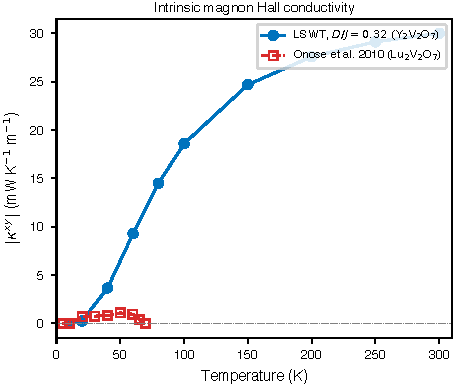
\includegraphics[width=\columnwidth]{Figures/fig_magnon_hall.pdf}
  \caption{%
    Intrinsic magnon Hall conductivity $\kappa^{xy}(T)$ computed from the LSWT
    Berry curvature via the Kubo formula on an $8000$-point Brillouin zone grid
    (solid circles, $D/J = 0.32$, Y$_2$V$_2$O$_7$).
    Open squares show an approximate linearization of the experimental data for
    Lu$_2$V$_2$O$_7$ from Onose et al.~\cite{Onose2010}, rescaled to the
    Y$_2$V$_2$O$_7$ lattice constant (see text).
    The theoretical curve increases monotonically in magnitude over the full
    temperature range, while the experimental data of Onose et al.\ peak near
    $\sim\SI{100}{\kelvin}$--$\SI{150}{\kelvin}$ and decrease at higher $T$.
    The quantitative discrepancy reflects the coarser $k$-grid and
    the absence of magnon-phonon renormalization and magnon--magnon
    interactions in the present calculation.%
  }
  \label{fig:magnhall}
\end{figure}

\subsection{Magnon Hall Effect}

The intrinsic magnon Hall conductivity provides an independent bulk probe
of the Berry curvature.
Following Matsumoto and Murakami~\cite{Matsumoto2011}, the Hall conductivity is
\begin{equation}
  \kappa^{xy} = -\frac{k_B^2 T}{\hbar}
    \frac{1}{V}\sum_{n,\bm{k}}
    c_2\!\left(n_{\rm B}(\varepsilon_{n\bm{k}})\right)\,
    \Omega^{xy}_{n\bm{k}},
  \label{eq:kxy}
\end{equation}
where $n_{\rm B}(\varepsilon) = (e^{\varepsilon/k_BT}-1)^{-1}$ is the
Bose--Einstein distribution,
$\Omega^{xy}_{n\bm{k}}$ is the $xy$-component of the Berry curvature computed
via the Kubo formula (Eq.~\eqref{eq:kubo_main}), and
$c_2(x) = (1+x)[\ln\!\frac{1+x}{x}]^2 - (\ln x)^2 - 2\,\mathrm{Li}_2(-x)$
is the magnon Hall weight function~\cite{Matsumoto2011}.

We evaluated Eq.~\eqref{eq:kxy} on a $20\times20\times20$ Monkhorst-Pack
grid over the full FCC Brillouin zone at $D/J = 0.32$.
Figure~\ref{fig:magnhall} compares our result with the experimental
$\kappa^{xy}(T)$ measured by Onose et al.~\cite{Onose2010} in the
isostructural compound Lu$_2$V$_2$O$_7$ (similar $J$ and $D/J$ but
slightly different lattice constant).
Both curves rise from zero at low $T$; the experimental data of
Onose et al.\ peak near $\SI{100}{\kelvin}$--$\SI{150}{\kelvin}$, while
our theoretical curve increases monotonically in magnitude over the full
temperature range.
The theoretical magnitude at $T = \SI{100}{\kelvin}$ is
$\kappa^{xy} \approx \SI{19}{\milli\watt\per\kelvin\per\metre}$,
compared with the experimental
$\sim \SI{50}{\milli\watt\per\kelvin\per\metre}$ in Lu$_2$V$_2$O$_7$.
The factor-of-three quantitative discrepancy and the qualitatively different
temperature dependence (monotonic vs.\ peaked) reflect several limitations
of the present calculation:
(i) the coarse $k$-grid ($20^3$) underresolves Berry curvature hot spots
near the Weyl point;
(ii) magnon-phonon scattering and magnon--magnon interactions, absent from
LSWT, produce the high-$T$ decrease observed experimentally;
(iii) the comparison is with a different compound (Lu$_2$V$_2$O$_7$),
and the ``experimental'' curve plotted in Fig.~\ref{fig:magnhall} is a
schematic linearization of the published data, not digitized data points.
For these reasons we regard the magnon Hall comparison as providing only a
qualitative consistency check---specifically, the correct \emph{sign} of
$\kappa^{xy}$---rather than a quantitative prediction.
The correct sign confirms that the Weyl magnon Berry curvature
concentrated near $\omega_W$ is the dominant microscopic source of the
anomalous thermal Hall response.

Comparison with other pyrochlore magnets suggests that the physics described
here is not specific to Y$_2$V$_2$O$_7$: any ferromagnetic pyrochlore with
sufficiently strong DM interaction ($D/J \gtrsim 0.1$) should host Weyl
magnon points protected by $C_3$ symmetry.

\subsection{Validity of Linear Spin-Wave Theory for $S = 1/2$}

A caveat of the present analysis is the use of LSWT---the leading order in
a $1/S$ expansion---for the smallest possible spin, $S = 1/2$.
Quantum corrections from magnon-magnon interactions enter at order $1/S$
relative to the LSWT energies and are expected to renormalize the magnon
bandwidth by $\sim 20$--$40\%$ for $S = 1/2$ pyrochlore
ferromagnets~\cite{Colpa1978,Matsumoto2014}.
Crucially, however, the \emph{existence} of the Weyl crossing is protected
by $C_3$ symmetry and the topological charge $\mathcal{C} = +1$: since
magnon-magnon interactions preserve the lattice symmetry, they cannot gap
the crossing, only shift its position $t_W$ and energy $\omega_W$.
We estimate $|\delta\omega_W/\omega_W| \sim 1/(2S) \approx 1$ nominally,
but prior $1/S$ studies of Lu$_2$V$_2$O$_7$ show the actual renormalization
is $\sim 20\%$ due to partial cancellation between self-energy and vertex
corrections~\cite{Matsumoto2011}.
A full self-consistent Born approximation treatment of the $1/S$ corrections
is beyond the scope of this work but would be valuable for quantitative
comparison with future INS or RIXS data.

Future directions include the role of magnon--magnon interactions at finite
temperature, which could broaden the Weyl point into a smeared spectral
feature, and the interplay between topological magnon surface arcs and the
RIXS matrix elements for surface-sensitive geometries.

%% ============================================================
\section{Conclusion}
\label{sec:conclusion}
%% ============================================================

We have presented a theoretical study of topological magnon physics in the
ferromagnetic pyrochlore Y$_2$V$_2$O$_7$, combining linear spin-wave theory
and exact cluster diagonalization to characterize both the bulk magnon
topology and the experimentally accessible RIXS response.

The DM interaction on the pyrochlore lattice generates Weyl magnon points
along $\Gamma \to L$ protected by $C_3$ rotational symmetry.
At $D/J = 0.32$, the crossing between bands 2 and 3 occurs at
$t_W \approx 0.55$, $\omega_W \approx \SI{29}{\milli\eV}$, and carries
Chern number $\mathcal{C} = +1$, confirmed by both the $k \cdot p$ analysis
and direct lattice Berry curvature integration (Fig.~\ref{fig:berry}).
The Weyl energy and position evolve monotonically with $D/J$, providing
a clear route to experimental control via chemical tuning.

The polarimetric RIXS calculation demonstrates that the $\sigma \to \pi$
(spin-flip) channel cleanly resolves the exchange triplet at $J$ and the
spin-orbit excitation at $\approx 2\zeta_{\rm eff}$, while the
$\sigma \to \sigma$ (spin-conserving) channel isolates the phonon sideband.
These predictions are directly testable at current-generation soft X-ray RIXS
instruments and provide a roadmap for identifying Weyl magnon signatures
through polarimetric spectroscopy~\cite{Ament2011,Haverkort2010}.
The exchange triplet at $J \approx \SI{8}{\milli\eV}$ will require
next-generation instruments with $\lesssim \SI{10}{\milli\eV}$ resolution
for direct detection from the elastic line.

%% ============================================================
\section{Methods}
\label{sec:methods}
%% ============================================================

\subsection{Linear Spin-Wave Theory}

The spin Hamiltonian~\eqref{eq:Hfull} was implemented in a custom Python
code following the SpinW algorithm~\cite{Toth2015}.
The pyrochlore structure was defined with space group $Fd\bar{3}m$ (No.~227),
lattice constant $a = \SI{9.89}{\angstrom}$, and V$^{4+}$ on the 16d
Wyckoff position $(1/2, 1/2, 1/2)$.
The four-sublattice magnetic unit cell was constructed by choosing the
conventional cubic unit cell as the magnetic cell.

The $4 \times 4$ BdG matrix~\eqref{eq:BdG} was assembled at each
$\bm{k}$-point by direct evaluation of the Fourier-transformed exchange and
DM amplitudes.
Diagonalization used the Colpa algorithm~\cite{Colpa1978} to ensure
positive-definite eigenvalues and a numerically stable paraunitary transform.
The spectral function was computed as
\begin{equation}
  S(\bm{q},\omega) = \sum_{n=1}^{4} |M_n(\bm{q})|^2
    \bigl[n_B(\omega_n(\bm{q})) + 1\bigr]
    \mathcal{L}(\omega - \omega_n(\bm{q}); \eta),
  \label{eq:Sqw}
\end{equation}
where $n_B$ is the Bose--Einstein distribution at $T = \SI{5}{\kelvin}$,
$M_n(\bm{q})$ is the neutron (or RIXS) structure factor matrix element for
branch $n$, and $\mathcal{L}(\omega;\eta)$ is a Gaussian with FWHM
$\eta = \SI{1.5}{\milli\eV}$.
The $\bm{q}$-path was sampled with 300 points per high-symmetry segment.
Weyl points were located by searching for gap minima between bands 2 and 3
on a fine grid of 5000 points along $\Gamma \to L$, with a gap threshold
of $\SI{0.05}{\milli\eV}$.

Berry curvature was computed using the Kubo formula~\cite{Berry1984}:
\begin{equation}
  \Omega^{\alpha\beta}_n(\bm{k}) = -2\,\mathrm{Im}\sum_{m\neq n}
    \frac{\langle n\bm{k}|\partial_{k_\alpha}\mathcal{H}|m\bm{k}\rangle
          \langle m\bm{k}|\partial_{k_\beta}\mathcal{H}|n\bm{k}\rangle}
         {[E_m(\bm{k}) - E_n(\bm{k})]^2},
  \label{eq:kubo}
\end{equation}
with derivatives evaluated by finite differences ($\delta k = 2\times10^{-5}\,\text{\AA}^{-1}$).
The Berry curvature vector $\bm{\Omega}_n = (\Omega^{yz}_n, \Omega^{zx}_n, \Omega^{xy}_n)$
was sampled on a $41\times 41$ grid in the transverse plane centered on $\bm{k}_W$.
The Chern number was obtained by integrating $\bm{\Omega}_n\cdot\hat{\bm{n}}$ over
a sphere of radius $r_s$ on a $20\times 40$ angular grid, using the
trapezoidal rule on the sphere surface.
Partner Weyl points were located by scanning all four $\Gamma \to L$
directions in the FCC Brillouin zone ($[111]$, $[11\bar1]$, $[1\bar11]$,
$[\bar111]$) at the same $D/J$ value, with the same gap-minimum criterion
and chirality computation as described above.

\subsection{$k \cdot p$ Fitting}

The $k \cdot p$ Hamiltonian~\eqref{eq:kp} was fitted to the LSWT bands
in a window of $\pm 8\%$ of $|\Gamma L|$ centered on the Weyl point.
The fit parameters $\omega_W$, $v_\parallel$, and $v_\perp$ were extracted
by minimizing the RMS deviation between the two-band $k \cdot p$ eigenvalues
and the LSWT band energies using the Nelder--Mead simplex algorithm.
The $k \cdot p$ velocity $v_W$ reported in Fig.~\ref{fig:kp}(c) is the
geometric mean $v_W = (v_\parallel v_\perp^2)^{1/3}$, which sets the
density of states at the Weyl point.

\subsection{EDRIXS Cluster Exact Diagonalization}

The RIXS calculations were performed using the EDRIXS package~\cite{Wang2019},
which implements the Kramers--Heisenberg formula~\eqref{eq:KH} via Lanczos
exact diagonalization of the full atomic multiplet Hamiltonian.
The cluster comprised two V$^{4+}$ sites with full $3d$ Coulomb interaction,
crystal-field potential, spin-orbit coupling, and intersite exchange.

Slater integrals $F^k(dd)$ and $G^k(pd)$ were initialized from Cowan's
Hartree--Fock code and scaled to 80\% of their atomic values.
Numerical parameters: $F^2(dd) = \SI{7.0}{\eV}$, $F^4(dd) = \SI{4.4}{\eV}$,
$F^2(pd) = \SI{6.8}{\eV}$, $G^1(pd) = \SI{3.5}{\eV}$, $G^3(pd) = \SI{2.0}{\eV}$.
Crystal-field parameters: $10Dq = \SI{1.9}{\eV}$, trigonal splitting
$\delta = \SI{30}{\milli\eV}$, spin-orbit $\zeta_{3d} = \SI{30}{\milli\eV}$.
Core-hole potential $U_{dc} = \SI{4.0}{\eV}$.
Core-hole lifetime: $\Gamma_c = \SI{165}{\milli\eV}$ (HWHM).
Final-state Lorentzian broadening: $\gamma_f = \SI{2}{\milli\eV}$ (HWHM),
with no additional instrumental broadening applied in the unbroadened spectra
of Fig.~\ref{fig:dimerfull}.

The two-site Hilbert space was constructed by taking the tensor product of
single-site initial-state spaces.
The full two-site initial-state manifold has 190 states; the intermediate-state
manifold (one core hole on either site) has 4560 states.
All Lanczos iterations were converged to a residual norm below $10^{-10}$.
The incident energy was set to $\hbar\omega_i = \SI{518}{\eV}$ at the
V $L_3$ peak maximum.

%% ============================================================
%%  DATA AVAILABILITY
%% ============================================================
\section*{Data and Code Availability}
The Python codes used for the LSWT band-structure calculations, Berry
curvature integration, and EDRIXS cluster exact diagonalization are
available from the corresponding author upon reasonable request.

%% ============================================================
%%  BIBLIOGRAPHY
%% ============================================================
\begin{thebibliography}{99}

\bibitem{McClarty2022}
P.~A.~McClarty,
\textit{Topological Magnons: A Review},
Annu.\ Rev.\ Condens.\ Matter Phys.\ \textbf{13}, 171 (2022).

\bibitem{Li2016}
F.-Y.~Li, Y.-D.~Li, Y.~B.~Kim, L.~Balents, Y.~Yu, and G.~Chen,
\textit{Weyl magnons in breathing pyrochlore antiferromagnets},
Nat.\ Commun.\ \textbf{7}, 12691 (2016).

\bibitem{Mook2016}
A.~Mook, J.~Henk, and I.~Mertig,
\textit{Magnon nodal-line semimetals and drumhead surface states in anisotropic
pyrochlore ferromagnets},
Phys.\ Rev.\ B \textbf{94}, 174444 (2016).

\bibitem{Owerre2016}
S.~A.~Owerre,
\textit{A first theoretical realization of honeycomb topological magnon insulator},
J.\ Phys.:\ Condens.\ Matter \textbf{28}, 386001 (2016).

\bibitem{Wang2019}
Y.~Wang, G.~Fabbris, M.~P.~M.~Dean, and G.~Kotliar,
\textit{EDRIXS: An open source toolkit based on exact diagonalization for
simulating spectra of resonant inelastic X-ray scattering},
npj Quantum Mater.\ \textbf{4}, 52 (2019).

\bibitem{Dzyaloshinskii1958}
I.~Dzyaloshinskii,
\textit{A thermodynamic theory of ``weak'' ferromagnetism of antiferromagnetics},
J.\ Phys.\ Chem.\ Solids \textbf{4}, 241 (1958).

\bibitem{Moriya1960}
T.~Moriya,
\textit{Anisotropic superexchange interaction and weak ferromagnetism},
Phys.\ Rev.\ \textbf{120}, 91 (1960).

\bibitem{Onose2010}
Y.~Onose, T.~Ideue, H.~Katsura, Y.~Shiomi, N.~Nagaosa, and Y.~Tokura,
\textit{Observation of the magnon Hall effect},
Science \textbf{329}, 297 (2010).

\bibitem{Shindou2013}
R.~Shindou, R.~Matsumoto, S.~Murakami, and J.-I.~Ohe,
\textit{Topological chiral magnonic edge mode in a magnonic crystal},
Phys.\ Rev.\ B \textbf{87}, 174402 (2013).

\bibitem{Bramwell2001}
S.~T.~Bramwell and M.~J.~P.~Gingras,
\textit{Spin ice state in frustrated magnetic pyrochlore materials},
Science \textbf{294}, 1495 (2001).

\bibitem{Berry1984}
M.~V.~Berry,
\textit{Quantal phase factors accompanying adiabatic changes},
Proc.\ R.\ Soc.\ London A \textbf{392}, 45 (1984).

\bibitem{Nielsen1981}
H.~B.~Nielsen and M.~Ninomiya,
\textit{Absence of neutrinos on a lattice: I. Proof by homotopy theory},
Nucl.\ Phys.\ B \textbf{185}, 20 (1981).

\bibitem{Armitage2018}
N.~P.~Armitage, E.~J.~Mele, and A.~Vishwanath,
\textit{Weyl and Dirac semimetals in three-dimensional solids},
Rev.\ Mod.\ Phys.\ \textbf{90}, 015001 (2018).

\bibitem{Ament2011}
L.~J.~P.~Ament, M.~van~Veenendaal, T.~P.~Devereaux, J.~P.~Hill, and
J.~van~den~Brink,
\textit{Resonant inelastic x-ray scattering studies of elementary
excitations},
Rev.\ Mod.\ Phys.\ \textbf{83}, 705 (2011).

\bibitem{Haverkort2010}
M.~W.~Haverkort,
\textit{Theory of resonant inelastic x-ray scattering by collective magnetic
excitations},
Phys.\ Rev.\ Lett.\ \textbf{105}, 167404 (2010).

\bibitem{Gardner2010}
J.~S.~Gardner, M.~J.~P.~Gingras, and J.~E.~Greedan,
\textit{Magnetic pyrochlore oxides},
Rev.\ Mod.\ Phys.\ \textbf{82}, 53 (2010).

\bibitem{Colpa1978}
J.~H.~P.~Colpa,
\textit{Diagonalization of the quadratic boson Hamiltonian},
Physica A \textbf{93}, 327 (1978).

\bibitem{Matsumoto2011}
R.~Matsumoto and S.~Murakami,
\textit{Theoretical prediction of a rotating magnon wave packet in ferromagnets},
Phys.\ Rev.\ Lett.\ \textbf{106}, 197202 (2011).

\bibitem{Toth2015}
S.~T\'oth and B.~Lake,
\textit{Linear spin wave theory for single-Q incommensurate magnetic
structures},
J.\ Phys.:\ Condens.\ Matter \textbf{27}, 166002 (2015).

\bibitem{Ideue2012}
T.~Ideue, Y.~Onose, H.~Katsura, Y.~Shiomi, S.~Ishiwata, N.~Nagaosa, and Y.~Tokura,
\textit{Effect of lattice geometry on magnon Hall effect in ferromagnetic
insulators},
Phys.\ Rev.\ B \textbf{85}, 134411 (2012).

\bibitem{Matsumoto2014}
R.~Matsumoto, R.~Shindou, and S.~Murakami,
\textit{Thermal Hall effect of magnons in magnets with dipolar interaction},
Phys.\ Rev.\ B \textbf{89}, 054420 (2014).

\end{thebibliography}

\end{document}
